\chapter{Eigenvalues of Slabs}

In this chapter we verify the correctness and examine the performance of the Rayleigh quotient fixed point methods for one-dimensional media such as slabs and one-dimensional spheres. In slab geometry, the phase space of the neutron transport equation is simplified with only one position variable $x$ and one angular variable $\mu$ defined as the $x$-direction cosine. For slab geometry, the alpha- and $k$-effective eigenvalue neutron transport equations are given by Eqn.~\ref{eq:1DAlphaSlab} and Eqn.~\ref{eq:1DkSlab}, respectively:

\begin{multline}
\bigg [ \mu \frac{\partial}{\partial x} + \frac{\alpha}{v(E)} + \sigma(x,E) \bigg ] \psi(x,\mu,E) \\ = \frac{\chi(E)}{2} \int_{0}^{\infty} \diff E' \nu(E') \sigma_{f}(x,E') \int_{-1}^{1} \diff \mu' \psi(x,\mu',E) \\ + \frac{1}{2} \int_{0}^{\infty} \diff E' \sigma_{s}(x, E' \rightarrow E) \int_{-1}^{1} \diff \mu' \psi(x,\mu',E),
\label{eq:1DAlphaSlab}
\end{multline}
\begin{multline}
\bigg [ \mu \frac{\partial}{\partial x}  + \sigma(x,E) \bigg ] \psi(x,\mu,E) \\ = \frac{1}{k} \frac{\chi(E)}{2} \int_{0}^{\infty} \diff E' \nu(E') \sigma_{f}(x,E') \int_{-1}^{1} \diff \mu' \psi(x,\mu',E) \\ + \frac{1}{2} \int_{0}^{\infty} \diff E' \sigma_{s}(x, E' \rightarrow E) \int_{-1}^{1} \diff \mu' \psi(x,\mu',E).
\label{eq:1DkSlab}
\end{multline}

Various homogeneous and heterogeneous slab geometry problems with vacuum boundary conditions were modeled in ARDRA. These slab media problems consist of multiplying and non-multiplying materials with thicknesses $\Delta$. Alpha- and $k$-effective eigenvalues were calculated and the number of transport sweeps compared to various methods such as the critical search method and the power method. To verify the correctness of the Rayleigh quotient fixed point method (RQFP), the method was compared to various methods such as Green's Function Method (GFM) and Direct Evaluation (DE) and compared to other discrete ordinate neutron transport codes such as PARTISN/DANT.

\section{One-Speed Verification}

For five one-speed non-multiplying slabs, calculated alpha-eigenvalues were benchmarked to the GFM \cite{kornreich_timeeigenvalue_2005}, described in Section~\ref{sec:CalcAlpha}. For these sets of problems, the neutron speed was set to $v = 1$ cm/s and the total cross section set to unity $\sigma = 1$ cm$^{-1}$. The slabs were purely scattering (Table~\ref{table:Betzler}). Problem thicknesses $\Delta$ were in mean free paths (mfps).

\begin{table}[H]
    \centering
    \caption{Non-Multiplying Homogeneous Slab Cross Sections (cm$^{-1}$)}
\label{table:Betzler}
    \begin{tabular}{*4c}
        \toprule
	$\sigma$ & $\nu \sigma_{f}$ & $\sigma_{s}$  & $v$ [cm/s] \\ 
        \midrule
	1.0 & 0.0 & 1.0 & 1.0 \\
        \bottomrule
    \end{tabular}
\end{table}

For multiplying media, 22 one-speed slabs of varying thickness $\Delta$ were examined and the Rayleigh quotient fixed point calculated alpha-eigenvalues were benchmarked to the GFM. The total cross section was set to unity and the slab neutron multiplication set to $\nu \sigma_{f} = 0.25$. The scattering cross section was set to $\sigma_{s} = 0.9$ cm$^{-1}$ (Table~\ref{table:Betzler2}).

\begin{table}[H]
    \centering
    \caption{Multiplying Homogeneous Slab Cross Sections (cm$^{-1}$)}
\label{table:Betzler2}
    \begin{tabular}{*5c}
        \toprule
	$\sigma$ & $\nu \sigma_{f}$ & $\sigma_{s}$ & $v$ [cm/s] \\ 
        \midrule
	1.0 & 0.25 & 0.9 & 1.0 \\
        \bottomrule
    \end{tabular}
\end{table}

Five one-speed heterogeneous slab problems consisting of two materials were examined and the Rayleigh quotient fixed point calculated alpha-eigenvalues compared to the GFM, direct evaluation (DE) \cite{modak_simple_2003}, and DANT/PARTISN \cite{alcouffe2005partisn}. With a fixed maximum medium width, material slabs of thickness $\Delta$ with cross sections as seen in Table~\ref{table:BetzlerHetero} were alternated until reaching the maximum fixed width. The impact of material widths on the alpha-eigenvalue was examined for this non-multiplying medium.

\begin{table}[H]
    \centering
    \caption{Non-Multiplying Heterogeneous Slab Material Cross Sections (cm$^{-1}$)}
\label{table:BetzlerHetero}
    \begin{tabular}{*6c}
        \toprule
	Material & $\sigma$ & $\nu \sigma_{f}$ & $\sigma_{s}$ & $v_{g}$ [cm/s] \\ 
        \midrule
	1 & 10.0 & 0.0 & 10.0 & 1.0 \\
	2 & 10.0 & 0.0 & 9.0 & 1.0 \\
	Homogeneous & 10.0 & 0.0 & 9.5 & 1.0 \\
        \bottomrule
    \end{tabular}
\end{table}

A two-region multiplying slab was examined with material properties as seen in Table~\ref{table:BetzlerHeteroMult}. The problem consisted of a 1.5 mfp region on the right and a 1.0 mfp region to the left. Both materials were multiplying and the system was supercritical \cite{kornreich_greens_1997}.

\begin{table}[H]
    \centering
    \caption{Multiplying Heterogeneous Slab Material Cross Sections (cm$^{-1}$)}
\label{table:BetzlerHeteroMult}
    \begin{tabular}{*6c}
        \toprule
	Material & $\sigma$ & $\nu \sigma_{f}$ & $\sigma_{s}$ & $v_{g}$ [cm/s] \\ 
        \midrule
	1 & 1.0 & 0.6 & 0.9 & 1.0 \\
	2 & 1.0 & 0.3 & 0.2 & 1.0 \\ 
        \bottomrule
    \end{tabular}
\end{table}

Four one-speed five region slab problems consisting of fuel, moderator, and absorber materials were examined and the Rayleigh quotient fixed point method alpha-eigenvalue compared to the GFM. The alpha-eigenvalue was calculated for different fuel width thicknesses with the fuel having $\nu \sigma_{f} = 0.3$ or 0.7. Cross sections for the three materials are seen in Table~\ref{table:BetzlerFive}.

\begin{table}[H]
    \centering
    \caption{Five Region Slab Material Cross Sections (cm$^{-1}$)}
\label{table:BetzlerFive}
    \begin{tabular}{*6c}
        \toprule
	Material & $\sigma$ & $\nu \sigma_{f}$ & $\sigma_{s}$ & $v_{g}$ [cm/s] \\ 
        \midrule
	Fuel & 1.0 & 0.3/0.7 & 0.8 & 1.0 \\
	Moderator & 1.0 & 0.0 & 0.8 & 1.0 \\ 
	Absorber & 1.0 & 0.0 & 0.1 & 1.0 \\ 
        \bottomrule
    \end{tabular}
\end{table}

\subsection{Non-Multiplying Homogeneous Slab}
For the one-speed, purely-scattering, homogeneous slabs of thicknesses $\Delta = 1.0$ to $\Delta = 25.0$ mfp with cross sections shown in Table~\ref{table:Betzler}, the Rayleigh quotient fixed point method showed good agreement with the GFM (Table~\ref{table:CompHomogScatt}). For $M = 500$ cells and $L = 64$ angular quadrature points, the subcritical alpha-eigenvalues matched within less than 0.1\% relative error. The greatest discrepancy between the two methods was for $\Delta = 1.0$ mfp. As the slab thickness gets smaller, the existence of a dominant alpha-eigenvalue is not assured and we begin to see this behavior. As the slab thickness increases, the number of transport sweeps necessary to converge the alpha-eigenvalue to a tolerance of $10^{-12}$ increases. However, the relative error between RQFP and the GFM decreases. 

\begin{table*}[t]
\centering\ra{1.3}
\caption{Comparison of RQFP- and GFM-calculated alpha-eigenvalues for a homogeneous scattering slab}
\label{table:CompHomogScatt}
\begin{tabular}{@{}cccc@{}}\toprule
& \multicolumn{3}{c}{Alpha-Eigenvalue/Percent Relative Error} \\
\cmidrule{2-4} $\Delta$ & RQFP & GFM & \% Relative Error \\
\midrule
%$\Delta$\\
1 & $-6.08420 \times 10^{-1}$ & $-6.08072 \times 10^{-1}$ & 0.057189 \\ 
5 & $-8.10966 \times 10^{-2}$ & $-8.10933 \times 10^{-2}$ & 0.004113 \\ 
10 & $-2.53506 \times 10^{-2}$ & $-2.53500 \times 10^{-2}$ & 0.002349 \\ 
20 & $-7.18015 \times 10^{-3}$ & $-7.17962 \times 10^{-3}$ & 0.007358 \\ 
25 & $-4.71736 \times 10^{-3}$ & $-4.71722 \times 10^{-3}$ & 0.002966 \\ 
\bottomrule
\multicolumn{4}{l}{$M = 500$, $L = 64$, Tolerance = $10^{-12}$} \\
\end{tabular}
\end{table*}

\subsection{Multiplying Homogeneous Slab}

For the material cross sections shown in Table~\ref{table:Betzler2}, one-speed homogeneous multiplying slabs of thicknesses of thickness $\Delta = 1.0$ to $\Delta = 50.0$ mfp showed good agreement between RQFP and the GFM with the exception of thin slabs. For thin slabs of up to width $\Delta = 1.0$ mfp, percent relative error was substantial. This is caused by the difficulty of numerically determining the alpha-eigenvalues for thin slabs. If the slab is thin enough, the existence of an alpha-eigenvalue is not assured. As the slab thickness increase, agreement was substantially better (Table~\ref{table:CompHomogMult}). 

For supercritical systems, the RQFP was compared to the critical search method (Table~\ref{table:CompMultSweeps}). The RQFP method substantially outperformed the critical search method in all cases. As the system became more supercritical, the number of transport sweeps necessary to converge increased for both methods. For the most supercritical slab ($\Delta = 50.0$ mfp), the number of sweeps necessary for the RQFP method to converge was less than the number of transport sweeps necessary for critical search to converge for the $\Delta = 4.0$ mfp case. Since the RQFP method requires no intermediate $k$-effective eigenvalue calculations, the method substantially reduced the number of transport sweeps necessary as there was no need to do multiple $k$-effective eigenvalue calculations to bracket the alpha-eigenvalue.
\begin{table*}[t]
\centering\ra{1.3}
\caption{Comparison of RQFP- and GFM-calculated alpha-eigenvalues for a homogeneous scattering multiplying slab}
\label{table:CompHomogMult}
\begin{tabular}{@{}cccc@{}}\toprule
& \multicolumn{3}{c}{Alpha-Eigenvalue/Percent Relative Error} \\
\cmidrule{2-4} $\Delta$ & RQFP & GFM & \% Relative Error \\
\midrule
%$\Delta$\\
0.25 & $-1.15480 \times 10^{0}$ & $-9.90300 \times 10^{-1}$ & 16.611352 \\ 
0.30 & $-1.06633 \times 10^{0}$ & $-9.74300 \times 10^{-1}$ & 9.446240 \\ 
0.35 & $-9.98584 \times 10^{-1}$ & $-9.49350 \times 10^{-1}$ & 5.186069 \\ 
0.40 & $-9.42114 \times 10^{-1}$ & $-9.17000 \times 10^{-1}$ & 2.738758 \\ 
0.45 & $-8.91833 \times 10^{-1}$ & $-8.79460 \times 10^{-1}$ & 1.406940 \\ 
0.50 & $-8.44920 \times 10^{-1}$ & $-8.38790 \times 10^{-1}$ & 0.730822 \\ 
0.75 & $-6.34756 \times 10^{-1}$ & $-6.34060 \times 10^{-1}$ & 0.109818 \\ 
1 & $-4.69398 \times 10^{-1}$ & $-4.69160 \times 10^{-1}$ & 0.050762 \\ 
2 & $-1.36335 \times 10^{-1}$ & $-1.36310 \times 10^{-1}$ & 0.018335 \\ 
3 & $-1.39888 \times 10^{-2}$ & $-1.39790 \times 10^{-2}$ & 0.070397 \\ 
4 & $4.36998 \times 10^{-2}$ & $4.37050 \times 10^{-2}$ & 0.011811 \\ 
5 & $7.54667 \times 10^{-2}$ & $7.54690 \times 10^{-2}$ & 0.003096 \\ 
6 & $9.48296 \times 10^{-2}$ & $9.48310 \times 10^{-2}$ & 0.001470 \\ 
7 & $1.07508 \times 10^{-1}$ & $1.07510 \times 10^{-1}$ & 0.002137 \\ 
8 & $1.16263 \times 10^{-1}$ & $1.16260 \times 10^{-1}$ & 0.002344 \\ 
9 & $1.22563 \times 10^{-1}$ & $1.22560 \times 10^{-1}$ & 0.002390 \\ 
10 & $1.27248 \times 10^{-1}$ & $1.27250 \times 10^{-1}$ & 0.001492 \\ 
15 & $1.39126 \times 10^{-1}$ & $1.39130 \times 10^{-1}$ & 0.002605 \\ 
20 & $1.43649 \times 10^{-1}$ & $1.43650 \times 10^{-1}$ & 0.000663 \\ 
30 & $1.47066 \times 10^{-1}$ & $1.47070 \times 10^{-1}$ & 0.002483 \\ 
40 & $1.48317 \times 10^{-1}$ & $1.48320 \times 10^{-1}$ & 0.001982 \\ 
50 & $1.48910 \times 10^{-1}$ & $1.48910 \times 10^{-1}$ & 0.000004 \\ 
\bottomrule
\multicolumn{4}{l}{$M = 500$, $L = 64$, Tolerance = $10^{-12}$} \\
\end{tabular}
\end{table*}

\begin{table*}[t]
\centering\ra{1.3}
\caption{Comparison of RQFP and Critical Search Sweeps for Homogeneous Multiplying Slabs}
\label{table:CompMultSweeps}
\begin{tabular}{@{}cccccc@{}}\toprule
& \multicolumn{2}{c}{Transport Sweeps} & & \multicolumn{2}{c}{Transport Sweeps} \\
\cmidrule{2-3} \cmidrule{5-6} $\Delta$ & RQFP & Critical Search \quad &  \Delta & RQFP & Critical Search\\
\midrule
%$\Delta$\\
4 & 56 & 21044 & 10 & 166 & 78002\\ 
5 & 70 & 33036 & 15 & 308 & 89627 \\
6 & 85 & 44655 & 20 & 495 & 97267 \\
7 & 103 & 55242 & 30 & 1002 & 98087 \\ 
8 & 122 & 63851 & 40 & 1682 & 106055 \\ 
9 & 143 & 71181 & 50 & 2530 & 113189 \\
\bottomrule
\multicolumn{6}{l}{$M = 500$, $L = 64$, Tolerance = $10^{-12}$} \\
\end{tabular}
\end{table*}

\subsection{Heterogeneous Media}

\begin{figure}[t]
	\centering
	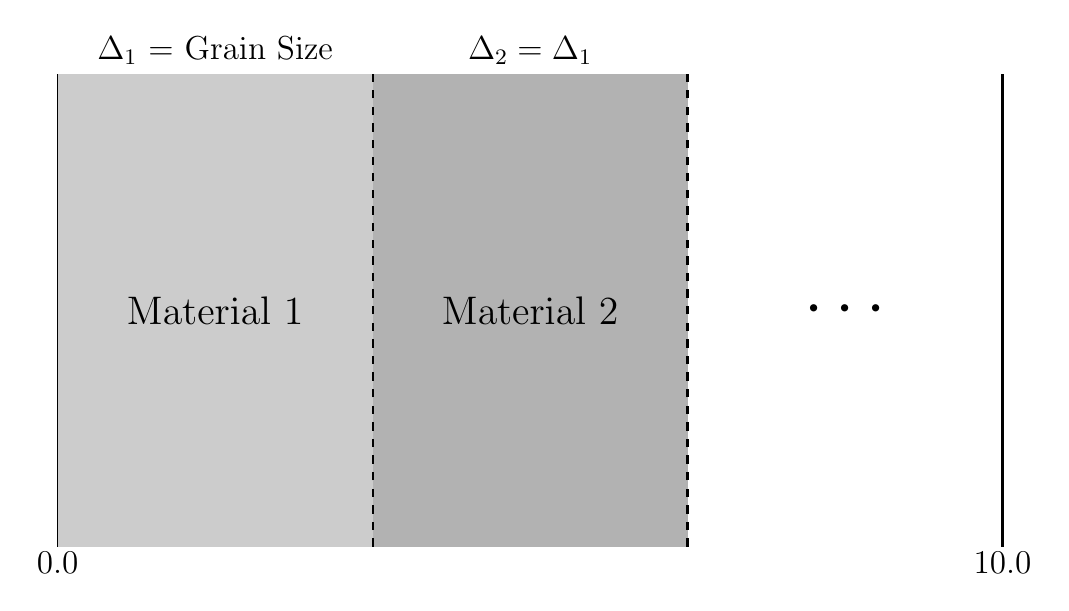
\begin{tikzpicture}
    \begin{scope}[thick,font=\scriptsize]

    \draw [-] (-3,-3) -- (-3,3) {};
    \draw [-] (9,-3) -- (9,3) {};
    
    \draw node at (-3,-3.2) {\large $0.0$};
    \draw node at (9,-3.2) {\large $10.0$};
    
    \fill[fill=black!20] (-3,-3) rectangle (1,3);
    \fill[fill=black!30] (1,-3) rectangle (5,3);
    
    \draw [dashed] (1,-3) -- (1,3) {};
    \draw [dashed] (5,-3) -- (5,3) {};
    
    \draw node at (-1,0) {\Large Material 1};
    \draw node at (3,0) {\Large Material 2};
    \draw node at (7,0) {\Huge{$\cdots$}};
    
    \draw node at (-1,3.3) {\large $\Delta_{1}$ = Grain Size}; 
    \draw node at (3,3.3) {\large $\Delta_{2} = \Delta_{1}$};

    \end{scope}
\end{tikzpicture}
	\label{fig:HeteroSlabDomain}
	\caption{Heterogeneous Slab Benchmark Problem Domain \cite{kornreich_timeeigenvalue_2005}}
\end{figure}

\textbf{Problem 6.1.3.1-Non-multiplying Heterogeneous Slab} For the subcritical heterogeneous medium shown in Figure~\ref{fig:HeteroSlabDomain}, five problems were constructed by varying the grain sizes of alternating slabs consisting of materials with the cross sections shown in Table~\ref{table:BetzlerHeteroMult}. The maximum width of the domain was fixed at 10.0 mfp. Grain sizes of 0.5, 1, 2.5, and 5 mfp were examined and their alpha-eigenvalue calculated by the RQFP method and compared to the GFM. One last case consisting of a homogenized material was considered. In all cases, the RQFP method showed good agreement with the GFM with percent relative error within 0.15\%.

\begin{figure}[t]
	\centering
	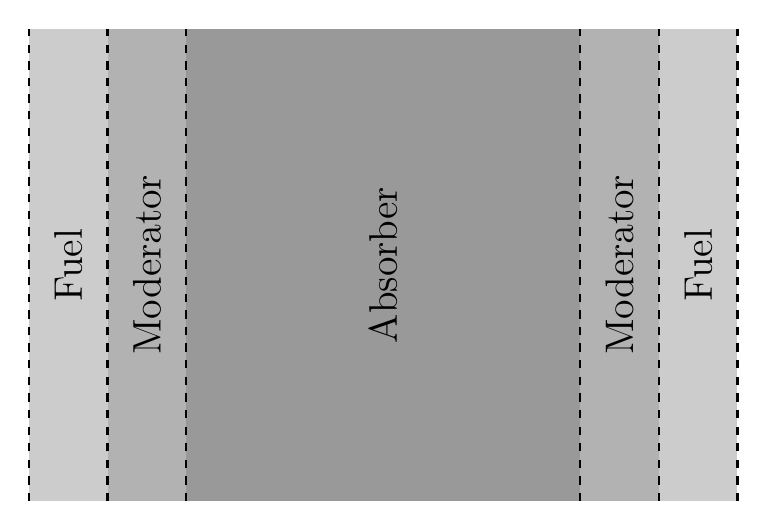
\begin{tikzpicture}
    \begin{scope}[thick,font=\scriptsize]
    
    \fill[fill=black!20] (-4.5,-3) rectangle (-3.5,3);
    \fill[fill=black!30] (-3.5,-3) rectangle (-2.5,3);
    \fill[fill=black!40] (-2.5,-3) rectangle (2.5,3);
        \fill[fill=black!30] (2.5,-3) rectangle (3.5,3);
            \fill[fill=black!20] (3.5,-3) rectangle (4.5,3);
    
    \draw [dashed] (-4.5,-3) -- (-4.5,3) {};
    \draw [dashed] (-3.5,-3) -- (-3.5,3) {};
    \draw [dashed] (-2.5,-3) -- (-2.5,3) {};
    \draw [dashed] (2.5,-3) -- (2.5,3) {};
   \draw [dashed] (3.5,-3) -- (3.5,3) {};
   \draw [dashed] (4.5,-3) -- (4.5,3) {};
   
   \draw node at (-4,0) {\Large \rotatebox[origin=c]{90}{Fuel}};
   \draw node at (-3,0) {\Large \rotatebox[origin=c]{90}{Moderator}};  
   \draw node at (-0,0) {\Large \rotatebox[origin=c]{90}{Absorber}};
   \draw node at (3,0) {\Large \rotatebox[origin=c]{90}{Moderator}};
   \draw node at (4,0) {\Large \rotatebox[origin=c]{90}{Fuel}};  

    \end{scope}
\end{tikzpicture}
	\label{fig:ThreeRegionProblem}
	\caption{Heterogeneous Slab Benchmark Problem Domain \cite{kornreich_timeeigenvalue_2005}}
\end{figure}

\begin{figure}
	\centering
	\begin{filecontents}{AlphaRQFP.dat}
x y
0.00E+00 1
1.50E-01 1.447247465
3.00E-01 1.755560563
4.50E-01 1.980425738
6.00E-01 2.125210861
7.50E-01 2.188765251
9.00E-01 2.169994135
1.05E+00 2.068765518
1.20E+00 1.885253322
1.35E+00 1.616038124
1.50E+00 1.208241837
1.60E+00 0.942444665
1.70E+00 0.777235239
1.80E+00 0.651820797
1.90E+00 0.551556358
2.00E+00 0.469075409
2.10E+00 0.399845272
2.20E+00 0.340724486
2.30E+00 0.289282031
2.40E+00 0.24323767
2.50E+00 0.198355012
\end{filecontents}

\begin{filecontents}{AlphaGFM.dat}
x    y
0    1
0.15 1.4573313
0.30 1.7677868
0.45 1.9942160
0.60 2.1400088
0.75 2.2040045
0.90 2.1851026
1.05 2.0831691
1.20 1.8983807
1.35 1.6272924
1.50 1.2166341
1.60 0.94899798
1.70 0.78264174
1.80 0.65635543
1.90 0.55539366
2.00 0.47233885
2.10 0.40262710
2.20 0.34309503
2.30 0.29129485
2.40 0.24493022
2.50 0.19900451
\end{filecontents}

\begin{tikzpicture}
\begin{axis}[
	xlabel=$x$ (MFP),
	ylabel=Scalar Flux $\phi(x)$
]
\addplot[color=red,mark=*] table {AlphaRQFP.dat};
\addlegendentry{RQFP}
\addplot[color=blue,mark=o] table {AlphaGFM.dat};
\addlegendentry{GFM}
\end{axis}
\end{tikzpicture}
	\label{fig:TwoRegionMultiply}
	\caption{Scalar Flux Results for Two-Region Multiplying Slab}
\end{figure}

\begin{figure}[t]
	\centering
	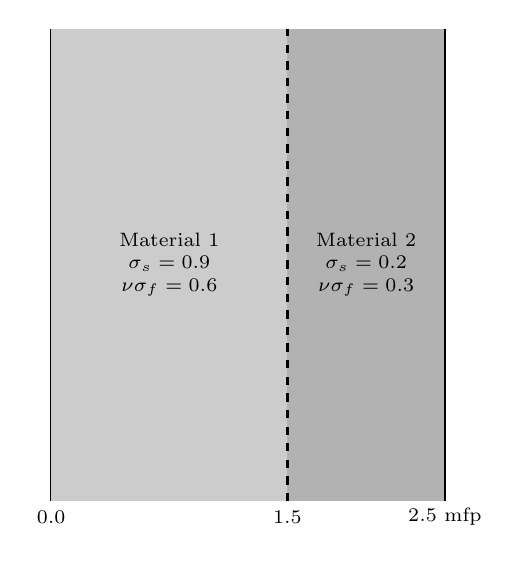
\begin{tikzpicture}[text centered]
    \begin{scope}[thick,font=\scriptsize]

    \draw [-] (-2.5,-3) -- (-2.5,3) {};
    \draw [-] (0.5,-3) -- (0.5,3) {};
    
    \draw node at (-2.5,-3.2) {$0.0$};
    \draw node at (2.5,-3.2) {$2.5$ mfp};
        \draw node at (0.5,-3.2) {$1.5$};
    
    \fill[fill=black!20] (-2.5,-3) rectangle (0.5,3);
    \fill[fill=black!30] (0.5,-3) rectangle (2.5,3);
    
    \draw [dashed] (0.5,-3) -- (0.5,3) {};
    \draw (2.5,-3) -- (2.5,3) {};
    
    \draw node [align=center] at (-1.0,0) {Material 1 \\ $\sigma_{s} = 0.9$ \\ $\nu \sigma_{f} = 0.6$};
    \draw node [align=center] at (1.5,0) {Material 2 \\ $\sigma_{s} = 0.2$ \\ $\nu \sigma_{f} = 0.3$};


    \end{scope}
\end{tikzpicture}
	\label{fig:HeteroSlabMult}
	\caption{Heterogeneous Multiplying Slab Benchmark Problem Domain \cite{kornreich_greens_1997}}
\end{figure}






\begin{table*}
\centering\ra{1.3}
\caption{Comparison of RQFP- and DANT/PARTISN-calculated alpha-eigenvalues for a multi-region scattering slab}
\begin{tabular}{@{}lccc@{}}\toprule
& \multicolumn{3}{c}{Alpha-Eigenvalue/Percent Relative Error} \\
\cmidrule{2-4} Grain Size & RQFP & DANT/PARTISN & \% Relative Error \\
\midrule
5 (2 slabs) & $-5.51528 \times 10^{-1}$ & $-5.50813 \times 10^{-1}$ & 0.129782 \\ 
2.5 (4 slabs) & $-7.03144 \times 10^{-1}$ & $-7.03134 \times 10^{-1}$ & 0.001470 \\ 
1 (10 slabs) & $-7.48808 \times 10^{-1}$ & $-7.48793 \times 10^{-1}$ & 0.001942 \\ 
0.5 (20 slabs) & $-7.57221 \times 10^{-1}$ & $-7.57199 \times 10^{-1}$ & 0.002882 \\ 
0 (homogeneous) & $-7.63513 \times 10^{-1}$ & $-7.63507 \times 10^{-1}$ & 0.000848 \\ 
\bottomrule
\multicolumn{4}{l}{$M = 500$, $L = 64$, Tolerance = $10^{-12}$} \\
\end{tabular}
\end{table*}

\begin{table*}
\centering\ra{1.3}
\caption{Comparison of RQFP- and GFM-calculated alpha-eigenvalues for a multi-region scattering slab}
\begin{tabular}{@{}lccc@{}}\toprule
& \multicolumn{3}{c}{Alpha-Eigenvalue/Percent Relative Error} \\
\cmidrule{2-4} Grain Size & RQFP & GFM & \% Relative Error \\
\midrule
5 (2 slabs) & $-5.51528 \times 10^{-1}$ & $-5.50812 \times 10^{-1}$ & 0.129964 \\ 
2.5 (4 slabs) & $-7.03144 \times 10^{-1}$ & $-7.03133 \times 10^{-1}$ & 0.001612 \\ 
1 (10 slabs) & $-7.48808 \times 10^{-1}$ & $-7.48792 \times 10^{-1}$ & 0.002075 \\ 
0.5 (20 slabs) & $-7.57221 \times 10^{-1}$ & $-7.57198 \times 10^{-1}$ & 0.003014 \\ 
0 (homogeneous) & $-7.63513 \times 10^{-1}$ & $-7.63507 \times 10^{-1}$ & 0.000848 \\ 
\bottomrule
\multicolumn{4}{l}{$M = 500$, $L = 64$, Tolerance = $10^{-12}$} \\
\end{tabular}
\end{table*}

\begin{table*}
\centering\ra{1.3}
\caption{Comparison of RQFP- and DE-calculated alpha-eigenvalues for a multi-region scattering slab}
\begin{tabular}{@{}lccc@{}}\toprule
& \multicolumn{3}{c}{Alpha-Eigenvalue/Percent Relative Error} \\
\cmidrule{2-4} Grain Size & RQFP & DE & \% Relative Error \\
\midrule
5 (2 slabs) & $-5.51528 \times 10^{-1}$ & $-5.51429 \times 10^{-1}$ & 0.017928 \\ 
2.5 (4 slabs)  & $-7.03144 \times 10^{-1}$ & $-7.03578 \times 10^{-1}$ & 0.061637 \\ 
1 (10 slabs) & $-7.48808 \times 10^{-1}$ & $-7.49672 \times 10^{-1}$ & 0.115312 \\ 
0.5 (20 slabs) & $-7.57221 \times 10^{-1}$ & $-7.58893 \times 10^{-1}$ & 0.220345 \\ 
0 (homogeneous) & $-7.63513 \times 10^{-1}$ & $-7.63640 \times 10^{-1}$ & 0.016569 \\ 
\bottomrule
\multicolumn{4}{l}{$M = 500$, $L = 64$, Tolerance = $10^{-12}$} \\
\end{tabular}
\end{table*}

%\begin{table*}
%\centering\ra{1.3}
%\begin{tabular}{@{}rrrr@{}}\toprule
%
%& \multicolumn{3}{c}{$w = 8$} \\
%\cmidrule{2-4} & $t=0$ & $t=1$ & $t=2$ \\
%\midrule$dir=1$\\
%$c$ & 0.0790 & 0.1692 & 0.2945 \\
%$c$ &  -0.8651& 50.0476& 5.9384 \\
%$c$ & 124.2756& -50.9612& -14.2721 \\
%$dir=0$\\
%$c$ & 0.0357& 1.2473& 0.2119 \\
%$c$ & -17.9048& -37.1111& 8.8591 \\
%$c$ & 105.5518& 232.1160& -94.7351\\
%\bottomrule
%\end{tabular}
%\caption{Caption}
%\end{table*}